\documentclass[UTF8]{ctexart}
\usepackage[table]{xcolor}
\usepackage{bm}
\usepackage{amssymb}
\usepackage{mathtools}
\usepackage{amsmath}
\usepackage{float}
\usepackage{rotating}
\usepackage{booktabs}
\usepackage{pdfpages}
\usepackage{subfigure}
\usepackage{mathtools}
\usepackage{amsmath}
\usepackage{listings}
\usepackage{fancybox}
%\usepackage{xcolor}
%\usepackage{colortbl}
\usepackage{diagbox}
\usepackage{amssymb}
\usepackage{warpcol}
\usepackage{lscape}
\usepackage[framemethod=tikz]{mdframed}
\usepackage{longtable,booktabs}

\title{\heiti 最优化第十六次作业}
\author{\kaishu 张晋15091060}
\begin{document}
\maketitle

\begin{enumerate}
\item[7.6]
\begin{enumerate}
\item
函数图像如下:
\begin{figure}[H]
\centering
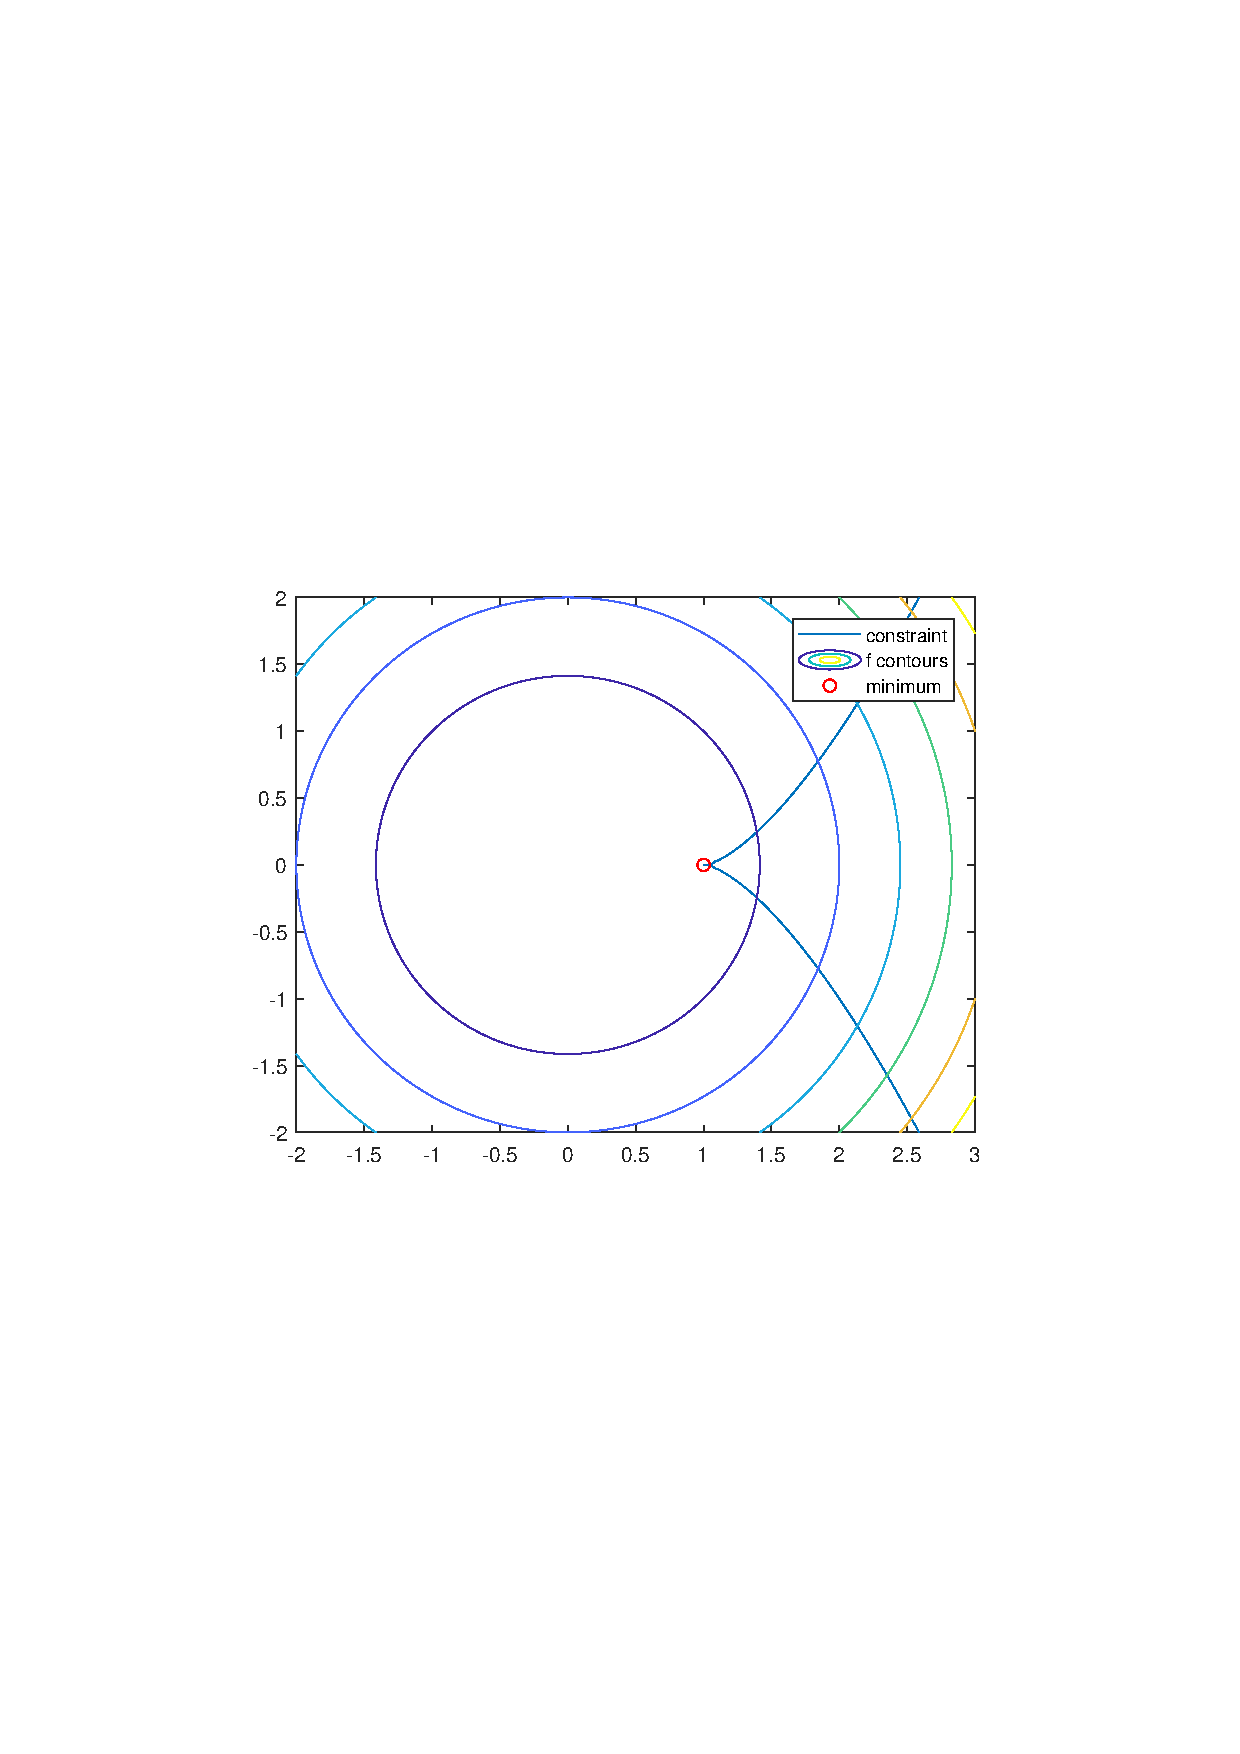
\includegraphics[width=8cm]{1.pdf}
\end{figure}

容易看出最优解为$(1,0)^T$.

消去$y$得到$f(x)={x^2} + {\left( {x - 1} \right)^3}$.

此时无极小点,因为消去$y$的同时少了约束条件:$x\geq 1$

消去$x$得到$f(y)=(y^{2/3}+1)^2+y^2$.

此时极小点为$y=0,x=1$.

\item
若存在KKT点,则必为局部极小点$(1,0)^T$,显然,存在线性化可行方向$p=(-1,0)^T$同时是下降方向,使得$\mathcal{F}\cap D \ne \emptyset$

故该问题没有KKT点。

在局部极小点$(1,0)^T$处,$a_1'=(0,0)^T$,故不满足LICQ条件
\end{enumerate}
\item[7.7]

函数图像如下:
\begin{figure}[H]
\centering
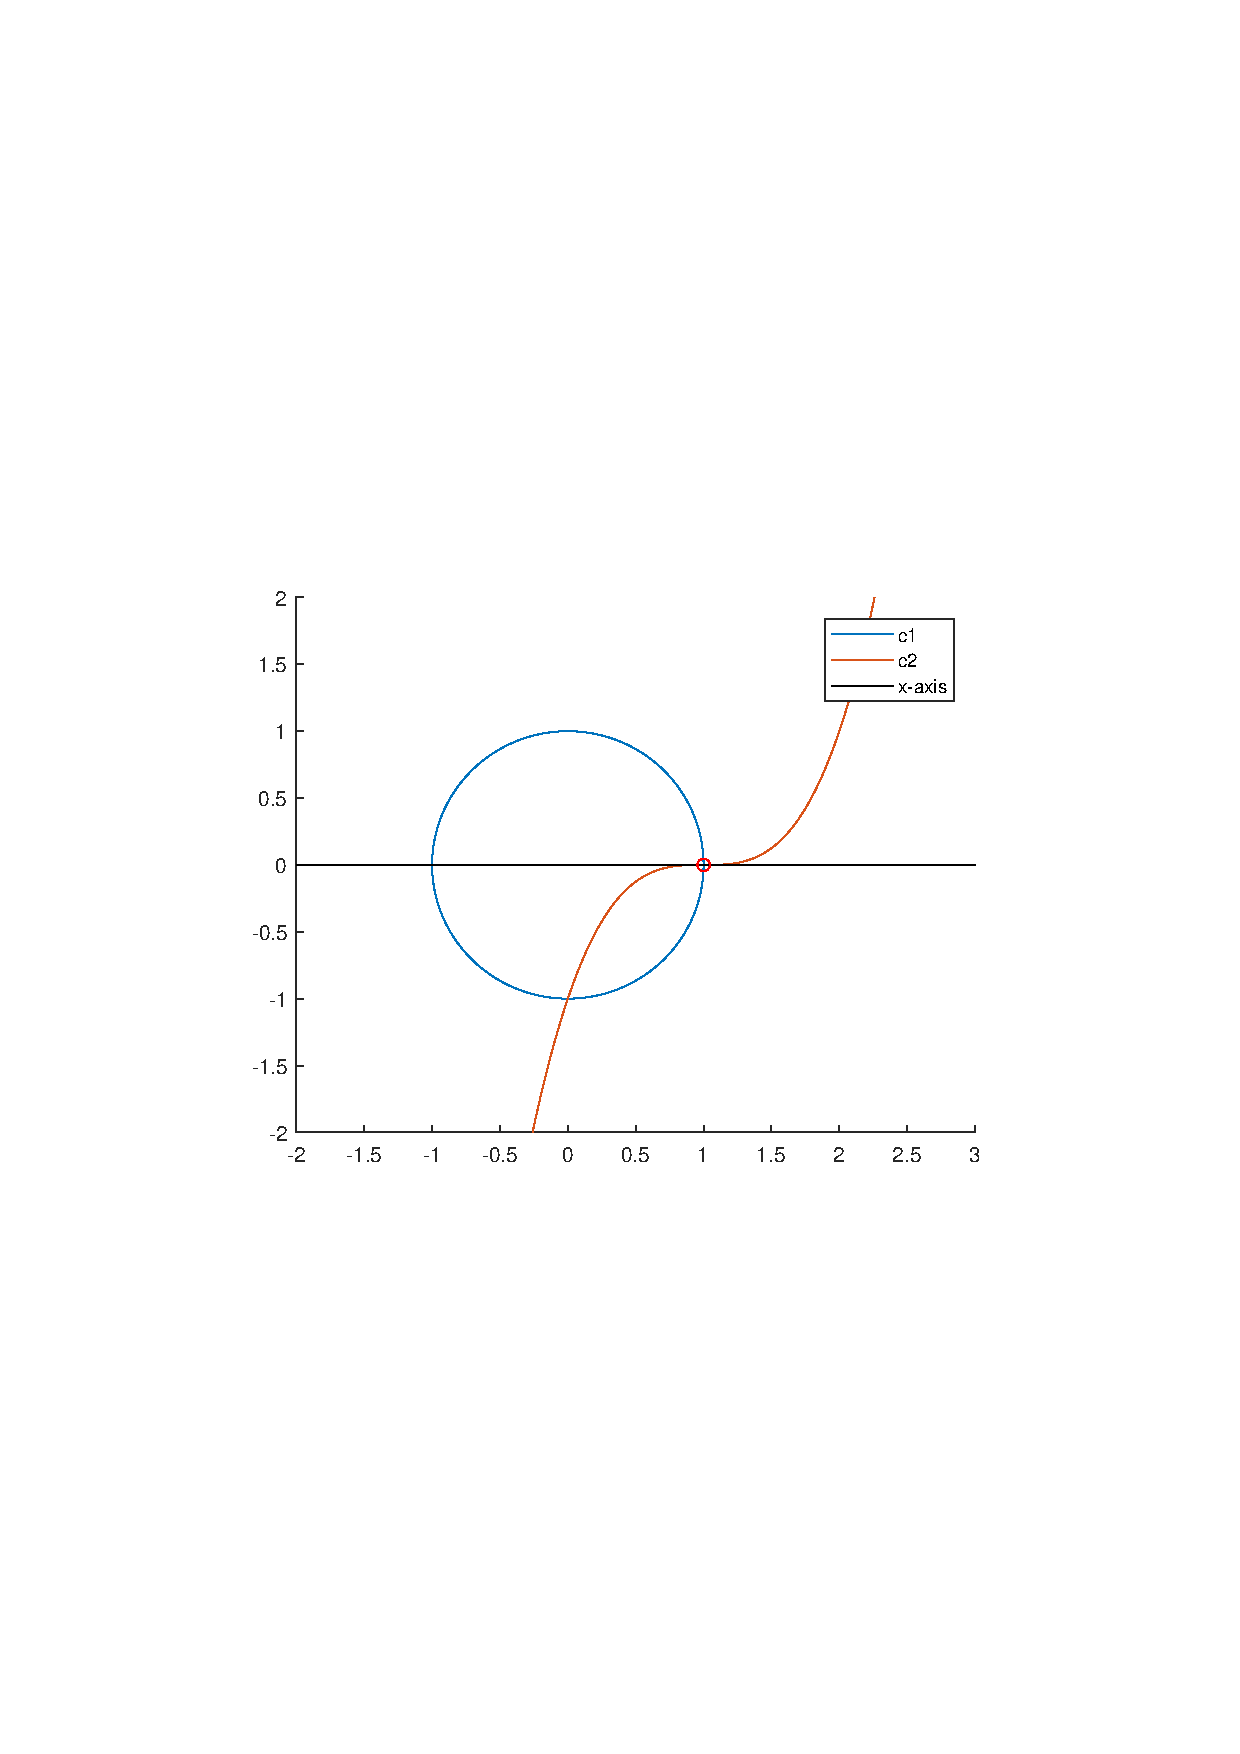
\includegraphics[width=10cm]{2.pdf}
\end{figure}
\begin{enumerate}
\item
观察得:在点$\bm{x}^{\star}$处,$a_1^{\star}//(1,0)^T,\quad a_2^{\star}//(0,-1)^T$,故线性无关,LICQ条件成立。

\item
因为点$\bm{x}^{\star}$是局部极小点,又满足LICQ条件,故其是KKT点。

由约束$c1$可知:$x_1<1$,故其是全局极小点。

\item
由于可行域为有界闭集,故一定能取到极小点,在该极小点处,由于约束条件都是线性的,满足LCQ条件,故为KKT点。

不一定,对于该问题可行域中可能存在多个局部极小点,它们都是KKT点,但不一定都是全局极小点,在$f$是凸函数的情况下,KKT点一定是最优解。
\end{enumerate}

\item[8.20]
将原问题表述成优化问题为:
\begin{alignat}{2}
min \quad & f(\bm{x})={x_1}^2+{x_2}^2+{x_3}^2 \nonumber\\
\mbox{s.t.}\quad
&-{x_1}-2{x_2}+{x_3}+4 \leq 0 \nonumber\\
&-{x_1}+{x_2}-{x_3}-2 \leq 0 \nonumber \\
\end{alignat}

\[\mathcal{L}(\bm{x},\lambda)={x_1}^2+{x_2}^2+{x_3}^2+\lambda_1(-{x_1}-2{x_2}+{x_3}+4)+\lambda_2(-{x_1}+{x_2}-{x_3}-2)\]

\[\nabla_{\bm{x}}\mathcal{L}(\bm{x},\lambda)=\begin{bmatrix}
2x_1-\lambda_1-\lambda_2\\
2x_2-2\lambda_1+\lambda_2\\
2x_3+\lambda_1-\lambda_2\\
\end{bmatrix}\]

\textbf{KKT条件:}
\begin{align}
2x_1-\lambda_1-\lambda_2&=0\\
2x_2-2\lambda_1+\lambda_2&=0\\
2x_3+\lambda_1-\lambda_2&=0\\
\lambda_1(-{x_1}-2{x_2}+{x_3}+4)&=0\\
\lambda_2(-{x_1}+{x_2}-{x_3}-2)&=0\\
-{x_1}-2{x_2}+{x_3}+4 &\leq 0 \nonumber\\
-{x_1}+{x_2}-{x_3}-2 &\leq 0 \nonumber \\
\lambda_1&\geq 0\nonumber\\
\lambda_2&\geq 0\nonumber\\
\end{align}

若这两个不等式约束都为积极约束,即:
\[-{x_1}-2{x_2}+{x_3}+4=0\]
\[-{x_1}+{x_2}-{x_3}-2=0\]

代入$f(\bm{x})$得:
\begin{align}
f(\bm{x})&=(-\dfrac{1}{3}x_3)^2+(2+\dfrac{2}{3}x_3)^2+x_3^2\\
&=\frac{14 }{9}x_3^2+\frac{8 }{3}x_3+4
\end{align}
故极值在$x_3=-6/7$时取到,此时$x_1=2/7,x_2=10/7$

代入得:$\lambda_2=-4/7$,故此解不是原问题的解

联立方程(2)(3)(4)(5)(6)解得:
\[\bm{x}^{\star}=(2/3,4/3,-2/3)^T,\quad \lambda^{\star}=(4/3,0)^T\]


\end{enumerate}
\end{document}
